% Couverture Thèse TPT Latex v2
% Fabrice Linot 04/12/11 

\documentclass[12pt,a4paper]{book}
\usepackage[left=1.3cm,top=0cm,right=1.3cm,bottom=1.2cm]{geometry}
\usepackage{graphicx}
\usepackage{eso-pic}
\usepackage{array}
\usepackage[english]{babel}
\usepackage[utf8x]{inputenc}
\usepackage[T1]{fontenc}
\usepackage{textcomp}
\usepackage{hyperref}
\usepackage{natbib}
\usepackage{helvet}	% or \usepackage{lmodern}

\usepackage[cmex10]{amsmath}
\usepackage{amssymb}
\usepackage{bbm}

% autoreject specific packages
\usepackage{enumitem}
\usepackage{multirow}
\usepackage{rotating}

% alphacsc specific packages
\usepackage{dsfont}
\usepackage{subfigure}
\usepackage{wrapfig}
\usepackage{algorithm}
\usepackage{algorithmic}
\usepackage{stmaryrd}

\usepackage{mathsymbols}

\renewcommand\textnumero{n$^{\textsf{{\tiny O}}}$}
\renewcommand{\familydefault}{\sfdefault}

\hypersetup{
    colorlinks,
    citecolor=red,
    filecolor=black,
    linkcolor=blue,
    urlcolor=blue
}

\usepackage{ifpdf}
\newcommand\BackgroundPic{
\ifpdf
	\includegraphics[height=\paperheight,width=\paperwidth]{cover_bg.pdf}
\else
	\includegraphics[height=\paperheight,width=\paperwidth]{cover_bg.pdf}
\fi}

\pagestyle{empty}

\begin{document}
\AddToShipoutPicture*{\BackgroundPic}
~

\begin{flushright}

\includegraphics[scale=0.45]{logo_TPT.pdf}

{\small {2015-ENST-00xx~~~~}}
\end{flushright}



%\vspace{0.cm}
\begin{center}
%


\includegraphics[scale=0.65]{logo_edite.pdf} \\
{\small {EDITE - ED 130}}


%
\vspace{.5cm}
%
%
%
%{\Large École doctorale \textnumero XX: texte}\\		% version une ligne
%{\Large École doctorale \textnumero XX:\\ texte}\\		% version deux lignes (changer les espaces en conséquence
%
%
%
\vspace{1.0cm}
%
%
%
{\LARGE {\bf Doctorat ParisTech}}\\
\vspace{1.1cm}
{\LARGE {\bf T H È S E}}\\
\vspace{0.5cm}
{\normalsize {\bf pour obtenir le grade de docteur délivré par}}\\
%
%
%
\vspace{.9cm}
%
%
%
%
{\LARGE {\bf TELECOM ParisTech}}\\
\vspace{0.6cm}
{\Large {\bf Spécialité Xxxx }}\\
%
%
%
\vspace{.8cm}
%
%
%
{\normalsize {\it présentée et soutenue publiquement par}}\\
\vspace{0.7cm}
{\Large {\bf Mainak JAS}}\\
\vspace{0.24cm}
{\normalsize le jour mois année}\\
%
%
%
\vfill
%
%
%
\textcolor[RGB]{191,18,56}{
\noindent
{\LARGE {\bf Advances in automating analysis of\\[.6cm]neural time series data}}\\
}
%
%
%
\vfill~\vfill
%
%
%
{\normalsize
\begin{tabular}{c}
Directeur de thèse:					{\bf Alexandre GRAMFORT}\\
Co-encadrement de la thèse:		{\bf Prénom NOM}
\end{tabular}
}
\end{center}
%
%
%
\vfill
%
%
%
\flushleft
\begin{minipage}{.9\textwidth}	% ou .91\textwidth si vous n'avez pas assez de place
{\bf Jury}\\
% Mme/M. Prénom NOM, Titre, Unité de recherche, Ecole 
{\bf Mme/M. Prénom NOM}, {\small Titre, Unité de recherche, Ecole}
	\hfill Fonction\\
{\bf Mme/M. Prénom NOM}, {\small Titre, Unité de recherche, Ecole}
	\hfill Fonction\\
{\bf Mme/M. Prénom NOM}, {\small Titre, Unité de recherche, Ecole}
	\hfill Fonction\\
{\bf Mme/M. Prénom NOM}, {\small Titre, Unité de recherche, Ecole}
	\hfill Fonction\\
{\bf Mme/M. Prénom NOM}, {\small Titre, Unité de recherche, Ecole}
	\hfill Fonction\\
{\bf Mme/M. Prénom NOM}, {\small Titre, Unité de recherche, Ecole}
	\hfill Fonction\\
{\bf Mme/M. Prénom NOM}, {\small Titre, Unité de recherche, Ecole}
	\hfill Fonction\\
{\bf Mme/M. Prénom NOM}, {\small Titre, Unité de recherche, Ecole}
	\hfill Fonction\\

\end{minipage}\\
%
%
%
\vspace{-.3cm}
%
%
%
{\centering
{\bf TELECOM ParisTech}\\
{\small école de l'Institut Mines-Télécom - membre de ParisTech}\\
{\tiny 46 rue Barrault 75013 Paris - (+33) 1 45 81 77 77 - www.telecom-paristech.fr}}
%
%
%
%
\newpage

%\renewcommand*\rmdefault{ptm}
\renewcommand{\familydefault}{\rmdefault}
%\linespread{1.5}
\setlength{\parskip}{1em}
\newcommand{\overbar}[1]{\mkern 1.5mu\overline{\mkern-1.5mu#1\mkern-1.5mu}\mkern 1.5mu}

\newpage
\vspace*{\fill}
\begin{center}
\textit{This dissertation is dedicated to the memory \\ 
of my friend and colleague Venkat Raghav Rajagopalan (1993 -- 2017).}
\end{center}
\vspace*{\fill}

\chapter*{Acknowledgements}
First and foremost, my gratitude goes out to Alexandre Gramfort: my advisor, mentor and friend. Through these years, Alex has inspired me with his technical knowledge, his vision for long term impact, philosophy of open science, and wisdom. He introduced me to the welcoming and progressive MNE community which ultimately formed my collaboration network. It is these interactions that often led to new research projects and ideas. A prime example of this is my work on \emph{autoreject} which developed out of my collaboration with Denis Engemann, a core contributor to MNE. It has been a pleasure working with Denis, as he shared his knowledge on the subtleties of MEG signal analysis and motivated me through our mini coding sprints. I would like to express my heartfelt thanks to Riitta Hari, Lauri Parkkonen, and Pavan Ramkumar who introduced me to the world of machine learning in neuroscience, and offered words of support and encouragement over the years. 

My gratitude goes out to Matti Hamalainen and Stephanie Jones for inviting me to Boston on our collaborative project. I thank my friend and former colleague, Teon Brooks for working with me on the BIDS project and on the realtime module in MNE, Eric Larson for sharing his extensive experience in MEG and signal processing, and the rest of the MNE team for making me believe in the power of open source. I am also grateful to Chris Gorgolewski and Russ Poldrack for inviting me to the BIDS coding sprint at Stanford. The visit was a very stimulating experience for me as well as a unique networking opportunity. I thank my advisor Alex, and Robert Gower for allowing me to take their optimization course, and for being incredibly patient with my questions. I am sure the skills I learned here will be useful for many years to come.

To my co-authors, I thank them for being so tolerant and supportive in our common projects. None of my papers could have been published without the teamwork and efforts put in by them. I am grateful to Umut \c{S}im\c{s}ekli and Tom Dupr\'{e} la Tour for spending their weekends and evenings with me to push forward our sparse coding project. I have benefited a lot from my collaboration with Jaakko Leppakangas who is perhaps one of the most efficient and productive engineers I have met. I am particularly indebted to my colleague, Yousra Bekhti for discussing tricky bugs at work, but more importantly for easing my difficulties with the French administration and with translation. I am grateful to Jean-Baptiste Schiratti for many stimulating technical conversations, and also for helping me with constructive feedback on my writing.

I thank my office mates for sharing the weekly seminars, the Monday cakes, and the latest free food event. I thank my collaborators and friends at the Neurospin laboratory for inviting me to their social events. It is here that I made many like-minded international friends. To my French teacher Françoise and our Tuesday French lunch group, I am immensely indebted. I thank my international friends: Bianca, David, Fosca, Gabriela, Magdalena, Sokhany, and Sophie. I thank my neighbours, my climbing partners, hiking group, and the \textit{desi} Indian community for making me feel home in France: Aakanksha, Anshuman, Chirag, Nilesh, Niraj, Pratheeban, Praveer, Raghav, Shabbir, Sidharth, and Vamsi.

All of this work would not have been possible without my family. My sister continues to surprise and inspire me with her sense of humour and adventure. Finally, I thank my parents for their continued moral support and motivation.

\vspace{3em}
April 12, 2018 \\
Paris

\tableofcontents
\listoffigures
\listoftables
\chapter{Introduction}

Understanding the human brain is one of the most significant challenges of the 21st century. The brain is responsible

\section{Modern brain imaging}

\begin{figure}[htb]
\begin{center}
   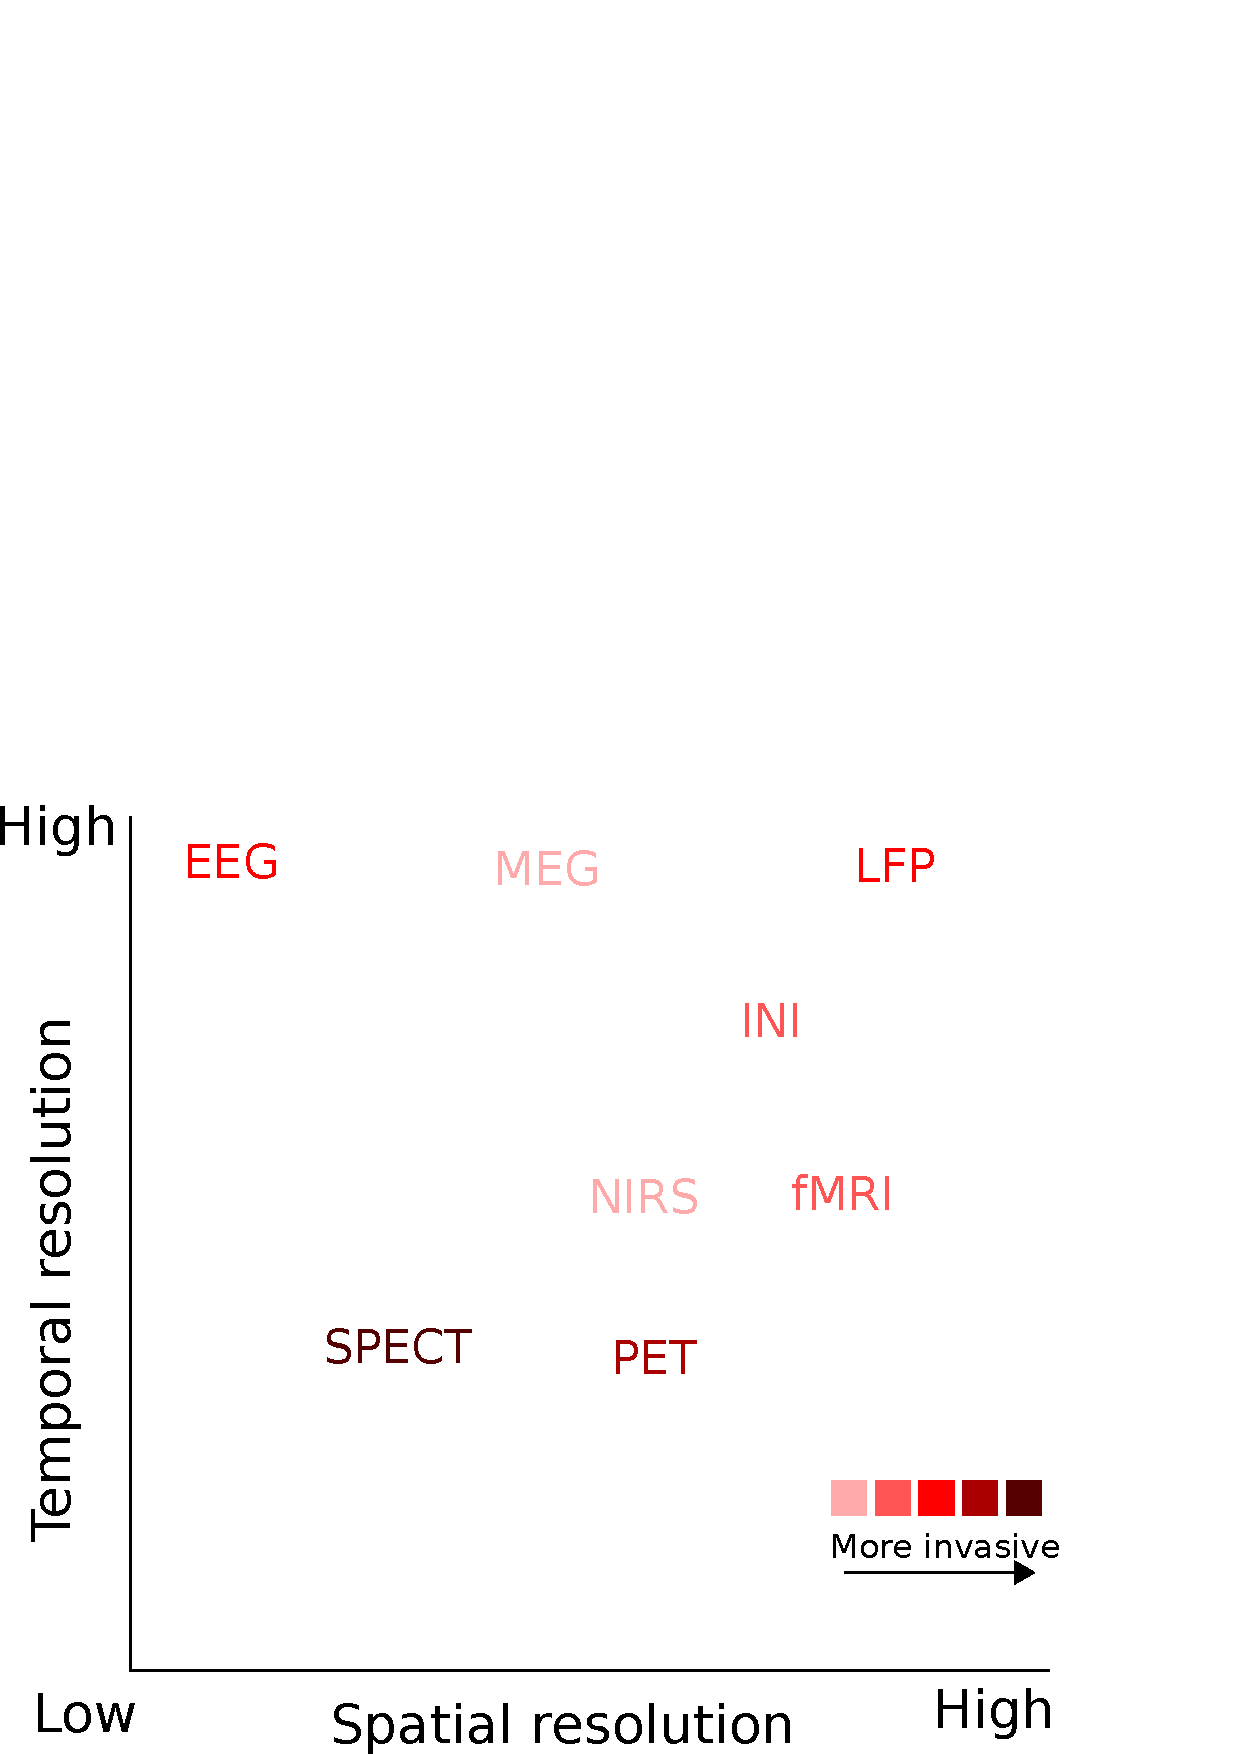
\includegraphics[width=0.4\linewidth]{figures/neuroimaging_methods.pdf}
\end{center}
   \caption{Various neuroimaging methods differ in terms of the information they measure. MEG=magnetoencephalography, EEG=electroencephalography, NIRS=near-infrared spectroscopy, PET=positron emission tomography, SPECT=single photon emission tomography, and INI=Inverse imaging, a method to speed up acquisition of fMRI images.}
   \label{fig:neuroimaging_methods}
\end{figure}

\section{The reproducibility crisis}

Even though thousands of papers are published every year about different aspects of the brain, our understanding of this complex organ has not scaled in proportion. A large part of the reason has been attributed to what is known as the replication crisis~\citep{ioannidis2005most, simmons2011false, button2013power}. Replication is closely related to the concept of reproducibility which refers to the idea that an experiment produces the same result when performed again under the same conditions. Replication is a stronger condition as it requires similar results or identical conclusion even if there are some minor variations in the experimental procedures. Progress in science rests on the reproducibility of experiments. In many fields, however, a large fraction of experiments cannot be reproduced. In psychology, for instance, it was estimated that over half of the papers were not reproducible~\citep{open2015estimating}, and even those reproduced tended to have a weaker effect size compared to the original study. 

This has led the field to look introspectively

preregistration, publishing negative results
 This is due to a number of reasons such as confirmation bias, pressure to publish and absence of incentives to publish negative results, ``p-hacking''~\citep{simmons2011false}. However, brain imaging has its own set of issues which can be linked to replication crisis:

% vul2009puzzlingly
% yendiki2014spurious

\begin{itemize}[noitemsep,nolistsep]
\item Multiple comparison
\item Differences in software
\item Complex pipelines~\citep{Carp2012289}
\item \emph{Power failure}, or the tendency to conduct studies using sample sizes thereby increasing the likelihood of a false discovery just by chance.
\item Head movements~\citep{yendiki2014spurious}
\item Lack of data
\end{itemize}

Lack of data and power failure are related

list the reasons for reproducibility crisis and how it's unique for neuroimaging as opposed to behavioral sciences

reverse inference

dead salmon~\citep{bennett2009neural}

\section{Data sharing}
The history of data sharing can be traced back to Newton and his theory of gravitation~\citep{pointofview2013}. Before Newton had developed his theory, another English astronomer, John Flamsteed had been appointed by the king to observe the stars and produce accurate charts for navigation in the seas. Over a period of 40 years, Flamsteed created a detailed catalogue that tripled the number of entries in the previously used sky atlas. When the great comet of 1680 appeared in the sky twice in close succession, Flamsteed used his data to postulate that it was not two comets but in fact the same comet which first went towards the sun and then turned away from it. Newton initially opposed this theory, but later changed his mind as he gained access to Flamsteed's unpublished catalogue. The comet had indeed turned out to be an important benchmark for Newton's theory of gravitation.

It is hard to imagine in this day and age that a theory as fundamental as the laws of gravitation could have been data driven. Today, data sharing is fundamental to reproducible science, but it also forms the cornerstone for learning better models and benchmarking new algorithms. If one follows the breakthroughs in the field of machine learning, for instance, it is predicated on the availability of data. It is an almost undisputed fact that the recent resurgence of deep learning owes in part at least, to the release of Imagenet~\citep{deng2009imagenet}. The same is true for Q learning in Atari games~\citep{watkins1992q, bellemare2013arcade}, natural language processing for language translation [ref], speech recognition [ref], and even the mixture of experts model~\citep{jacobs1991adaptive} for IBM Watson~\citep{ferrucci2010building}. If such datasets were available in neuroscience, we would be able to tease apart even subtle effects that were not possible before with smaller sample sizes.

Of course, neuroscientists are beginning to realize the importance of sharing data. In recent times, neural data has started being shared through international consortiums~\citep{van2013wu, ollier2005uk} and data repositories~\citep{poldrack2013toward, gorgolewski2015neurovault}. While in the case of Newton, he gained access to the catalogue without permission, today it is possible to publish dataset papers in targeted journals so as to assign the credit where it is due.
Data sharing is beneficial not just from the perspective of replication but also from an economic perspective. Rather than collect new data for every new hypothesis, researchers can now reuse existing data for answering their hypotheses.

\subsection{Brain Imaging Data Structure}

While data sharing in neuroscience is on the rise, the amount of data reuse is still limited. For instance, since the release of the Human Connectome Project (HCP) [ref -- meg one] data in 2013 [check], there have been only one or two documented cases of reusing the MEG data. Even in these cases, the effort has mostly been to reproduce rather than test new hypotheses. This brings us to a crucial point: dataset sharing is not a panacea as the tools, skills and resources to process such large datasets is currently missing. Perhaps the most important roadblock is standardization of metadata. 

Neuroimaging experiments are often complicated involving different paradigms (auditory, visual, somatosensory \emph{etc.}), different acquisition parameters (sampling frequency, number of sensors and their location, measurement device \emph{etc.}), and [subject's gender, age etc]. As if this weren't complicated enough, often intermediate results from the data are sometimes shared as well owing to the long preprocessing time. The data itself could be stored in 10--20 different file formats depending on the device used for acquisition. Therefore, it is almost a guaranteed fact that certain parameters will be missing or differently recorded when comparing across measurement sites.

A graduate student or postdoc who has newly started analyzing the data will be unable to make any progress unless all these different parameters are known beforehand. Combining different datasets, a first step towards making larger datasets, is almost out of question. To appreciate the importance of standardization, let us consider as a simpler example of the toy. Imagine, instead of the clocks that we know today, we had clocks that were nonstandard as in Figure [].

clock image [ref to design of everyday things]

Even though, it is easy to infer the time, it disturbs us. The reason is that we are used to reading clocks where the 12 o' clock mark is fixed at the top and the direction of motion is \emph{clockwise}. Indeed,

If we are to ever hope for crowdsourcing neural data acquisition, the first step must be standardizing the data formats.

\section{Automation}
Back in 2014, Nature published a bold article~\citep{hayden2014automated} which described a vision for the future: ``solving the problem of bringing McDonald's-like efficiency to scientists''. This would in turn lead to cheaper, more efficient and reliable research. While it goes on to describe many biology labs which are automating experiments, the benefits of automation in the neuroimaging community are yet to be widely recognized. But what are the opportunities for automation in the context of neuroimaging? Let us list down some of them:
\begin{itemize}[noitemsep,nolistsep,nosep]
\item \textbf{Data organization:} Neuroimaging data can often run into many Terabytes with intermediate files at different stages of processing. Keeping track of this heterogeneous data manually can be a challenging process.
\item \textbf{Parameter tuning:} Most algorithms, although automated, require hyperparameters to be tuned. This could be the number of trials to perform in an experiment, the number of components to select in a \ac{PCA} decomposition, or the regularization parameter in inverse solvers.
\item \textbf{Annotation and labeling:} The challenge of neuroimaging data is that it is often unlabeled. As reliable annotations can be performed only by experts, crowdsourcing is often not a possibility. The alternative is to automatically label different types of signals.
\item \textbf{Reporting and quality control:} Automated Statistician . \ac{MNE} web report
\end{itemize}
Ultimately, this will lead to higher quality of 

Efficiency, it turns out, is not simply a matter of scale. Even for moderately sized experiments,

% automated statistician
%
% This subjectivity can lead to studies which are not reproducible unless every single detail was carefully documented. Even then, it does not rule out a potential confirmation bias: the tendency to favor processing steps which leads one to confirm the hypothesis being tested rather than reject it.

data revolution


data sharing, data standards, open source

\subsection{Janitor work}

One of the biggest roadblocks to large scale analysis is what is known as `janitor work': the effort required to standardize a dataset before it is actually usable. In the context of neuroimaging, this can involve organizing files at different stages of processing, manually inspecting the data, annotating segments which contain artifacts, and even removing outlier subjects from the analysis. Merely based on anecdotal reports, we can conclude that this can take up to a week of time even for a moderately sized study of 10--20 subjects.
%If at some point, the researcher realized that a certain parameter early in the pipeline needed to be changed, this would entail redoing all the subsequent steps in the pipeline, including the manual processing. 
In addition to the cost of human labor, one cannot ignore the subjectivity that these steps produces which can be problematic for reproducibility. As the number of datasets shared increases and neuroscientists are forced to confront statistically rigorous approaches to data analysis, the time is ripe to automate as many steps of the pipeline as possible.

\section{Representation learning}

\section{Contributions}
In this thesis, I attempt to synthesize the lessons learned from analysing public neuroimaging data with open source software. To this effect, I participated in an effort to create an MEG standard for the Brain Imaging Data Structure (BIDS). I wrote the validator which helped create the MEG-BIDS compatible example datasets. As a long time contributor to MNE [ref], I led an effort to reanalyze a simple dataset for a reproducible group study. At the same time, we realized that reproducibility cannot be attained unless all steps of analysis pipeline are automated. This led us to develop a fully automated algorithm for artifact rejection and repair [ref]. Finally, we develop algorithms to learn new undiscovered motifs automatically from neural time series data. 

\subsection*{Journal publications}
\bibentry{jas2017autoreject} \\ \\
\bibentry{jas2017mne} \\ \\
\bibentry{galan2017meg}

\subsection*{Conference publications}
\bibentry{jas2016automated} \\ \\
\bibentry{jas2017learning}
\chapter{A reproducible M/EEG group study}
% autoreject
\input{chapters/3-1-autoreject_introduction.tex}
\section{Materials and methods}
%
We will first describe how a cross-validation procedure can be used to set peak-to-peak rejection thresholds globally (\textit{i.e.} same threshold for all sensors). This is what we call \textit{autoreject (global)}.

\subsection{Autoreject (global)}
\label{sec:auto_global}
We denote the data matrix by $X \in \real^{N \times P}$ with $N$ trials and $P$ features. These $P$ features are the $Q$ sensor-level time series, each of length $T$ concatenated along the second dimension of the data matrix, such that $P=QT$. We divide the data into $K$ folds (along the first dimension) with training set indices $\mathcal{T}_{k}$ and validation set indices $\mathcal{V}_{k}=[1..N] \setminus {\mathcal{T}_k}$ for each fold $k$ $(1 \leq k \leq K)$. For simplicity of notation, we first define the peak-to-peak amplitude for the $i$th trial and $j$th sensor as the difference between the maximum and the minimum value in that time series:
\begin{equation}
\mathcal{A}_{ij} = \max_{(j-1)T+1 \leq t \leq jT} (X_{it}) - \min_{(j-1)T+1 \leq t \leq jT} (X_{it}) \enspace .
\end{equation}
The good trials $\mathcal{G}_k$ where the peak-to-peak amplitude $\mathcal{A}_{ij}$ for any sensor does not exceed the candidate threshold $\tau$ are computed as
\begin{equation}
\mathcal{G}_k = \{i \in \mathcal{T}_{k} \suchthat \max_{1 \leq j \leq Q} \mathcal{A}_{ij} \leq \tau\}.
\end{equation}
By comparing the peak-to-peak threshold with the maximum of the peak-to-peak amplitudes, we ensure that none of the sensors exceed the given threshold. Once we have applied the threshold on the training set, it is necessary to evaluate how the threshold performs by looking at new data. For this purpose, we consider the validation set. Concretely speaking, we propose to compare the mean $\overbar{X_{\mathcal{G}_k}}$ of good trials in the training set against the median $\widetilde{X_{\mathcal{V}_k}}$ of all trials in the validation set. Using root mean squared error (RMSE) the mismatch $e_{k}(\tau)$ reads as:
\begin{equation}
 e_{k}(\tau) = \fro{\overbar{X_{\mathcal{G}_k}} - \widetilde{X_{\mathcal{V}_k}}}.
\label{eq:err} 
\end{equation}
Here, $\fro{\cdot}$ is the Frobenius norm. The rationale for using the median in the validation set is that it is robust to outliers. Indeed, it is far less affected by high-amplitude artifacts than a classical mean. The threshold with the best data quality (lowest mismatch $e_{k}(\tau)$) on average across the $K$ folds is selected as the optimal threshold. In practice $\tau$ is taken in a bounded interval $[\tau_{\min}, \tau_{\max}]$:
%
\begin{equation}
\tau_{\star} = \underset{\tau \in [\tau_{\min}, \tau_{\max}]} \argmin \frac{1}{K} \sum_{k=1}^{K}  e_{k}(\tau)
\label{eq:best_th}
\end{equation}
Note, that $\widetilde{X_{\mathcal{V}_k}}$ does not depend on $\tau$. Indeed, it would not be wise to restrict the validation set to good trials according to the value of $\tau$. As $\tau$ varies, it would lead to a variable number of validation trials, which would affect the comparison of RMSE across threshold values. The idea of using the median in the context of cross-validation has been previously proposed in the statistics literature in order to deal also with outliers~\citep{leung2005cross,de2003robust}.

Figure~\ref{fig:cross_val} shows how the average RMSE changes as the threshold varies for the MNE sample dataset~\citep{gramfort2013meg,mne}. At low thresholds, our model underfits as it drops most of the trials in the data resulting in a noisy average. On the other hand, at high thresholds, the model overfits retaining all the trials in the data including the high-amplitude artifacts. Here the candidate values of $\tau$ were taken on a grid. More details on how to solve \eqref{eq:best_th} will be given in Section~\ref{sec:bayesian_opt}.

\subsection{Autoreject (local)}
\label{sec:auto_local}

\begin{figure}[t]
	\centering
	\includegraphics[width=0.5\linewidth]{figures/figure3.pdf}
    \caption[A schematic diagram explaining how \emph{autoreject (local)} works.]{A schematic diagram explaining how \emph{autoreject (local)} works. (A) Each cell here is an element of the indicator matrix $C_{ij}$ described in Section~\ref{sec:auto_local}. Sensor-level thresholds are found and bad segments are marked for each sensor. Bad segments shown in red are where $C_{ij}=1$ (B) Trials are rejected if the number of bad sensors is greater than $\kappa$ and otherwise, the worst $\rho$ sensors are interpolated.}
    \label{fig:schematic}
\end{figure}

A global threshold common to all sensors, however, suffers from limitations. A common case of failure is when a single sensor is affected (locally or globally) by high-amplitude artifacts. In this case, $\max_{j} \mathcal{A}_{ij}$, which would be the peak-to-peak amplitude that is compared to the threshold, comes from this bad sensor. If the sensor is not repaired or removed, we might end up rejecting a large fraction of otherwise good trials, just because of a single bad sensor. This is certainly not optimal. In fact, a possibly better solution is to replace the corrupted signal in the sensor by the interpolation of the signals in the nearby sensors. A second observation is that sensors can have very different ranges of amplitudes depending on their location on the scalp. A threshold tuned for one sensor may not work as effectively for another sensor. Both of these observations are motivations for estimating rejection thresholds for each sensor separately.

Once we define sensor-wise rejection thresholds $\tau_{\star}^{j}$, we can define an indicator matrix $C_{ij} \in \{0, 1\}^{N \times Q}$ which designates the bad trials at the level of individual sensors. In other words, we have:
\begin{equation}
C_{ij} = \begin{cases} 
0, & \text{if } \mathcal{A}_{ij} \leq \tau^{j}_{\star} \\
1, & \text{if } \mathcal{A}_{ij} > \tau^{j}_{\star}
\end{cases}
\end{equation}
The schematic in Figure~\ref{fig:schematic}A shows a cartoon figure for this indicator matrix $C_{ij}$. Now that we have identified bad sensors for each trial, one might be tempted to interpolate all the bad sensors in each trial. However, it is not as straightforward since in some trials, a majority of the sensors may be bad. These trials cannot be repaired by interpolation and must be rejected. In some other cases, the number of bad sensors may not be large enough to justify rejecting the trial. However, it might already be too much to interpolate all the sensors reliably. In these cases, a natural idea is to pick the worst few sensors and interpolate them. This suggests an algorithm as described in Figure~\ref{fig:schematic}B. Reject a trial only if most sensors ``agree'' that the trial is bad, otherwise interpolate as many sensors as possible. We will denote by $\kappa$ the maximum number of bad sensors in a non-rejected trial and by $\rho$ the maximum number of sensors that can be interpolated. Note that $\rho$ is necessarily less than $\kappa$. The interpolation scheme for EEG uses spherical splines~\citep{perrin1989spherical} while for MEG it uses a Minimum Norm Estimates formulation with spherical harmonics~\citep{hamalainen1994interpreting}. The implementation is provided by MNE-Python~\citep{gramfort2013meg}.

The set of good trials $\mathcal{G}^{\kappa}_k$ in the training set $\mathcal{T}_k$ can therefore be written mathematically as:
%
\begin{equation}
\mathcal{G}^{\kappa}_{k} = \{i \in \mathcal{T}_k \suchthat \sum_{j=1}^{Q} C_{ij} < \kappa \} \enspace .
\end{equation}
%
In the remaining trials, if $\rho < \kappa$, one needs to define what are the worse $\rho$ sensors that shall be interpolated. To do this we propose to rank the sensors for ``badness'' according to a score. A natural strategy to set the score is to use the peak-to-peak amplitude itself:
%
\begin{equation}
s_{ij} = \begin{cases}
\mathcal{A}_{ij} & \text{if } C_{ij} = 1 \\
-\infty & \text{if } C_{ij} = 0
\end{cases}
\label{eq:score}
\end{equation}

Higher the score $s_{ij}$, the worse is the sensor. The $-\infty$ score is for ignoring the good sensors in the subsequent step. The following strategy is used for interpolation.
%
%
If the number of bad sensors $\sum_{j'=1}^{Q} C_{ij'}$ is less than $\rho$ we will interpolate all of them. Otherwise, we will interpolate the $\rho$ sensors with the highest scores.
In other words, we interpolate at most $\mathrm{min}(\rho, \sum_{j'=1}^{Q} C_{ij'})$ sensors.
%
%
%
%
%
%
%
%
%
%
%

Denoting by $X^{\rho}_{\mathcal{G}^{\kappa}_k}$ the data in the training set after rejection and cleaning by interpolation, the RMSE averaged over $K$ folds for the parameter pair $(\rho, \kappa)$ therefore becomes:
%
\begin{equation}
\overbar{e}(\rho, \kappa) = \frac{1}{K} \sum_{k=1}^{K} \fro{\overbar{X^{\rho}_{\mathcal{G}^{\kappa}_k}} - \widetilde{X_{\mathcal{V}_k}}}
\end{equation}
where $\fro{\cdot}$ is the Frobenius norm.
Finally, the best parameters $\rho_{*}$ and $\kappa_{*}$ are estimated using grid search~\citep{hsu2003practical}.
%

\subsubsection{Data augmentation}
\label{sec:data_augmentation}

\begin{figure}[ht!]
    \centering
    \includegraphics[width=0.7\linewidth]{figures/figure2.pdf}
    \caption[Sequential Bayesian optimization cross-validation curves]{(A) and (B) The cross-validation curve obtained with sequential Bayesian optimization (see Section~\ref{sec:bayesian_opt} for an explanation) for a regular (MEG 2523) and a globally bad sensor (MEG 2443) from the MNE sample dataset. The mean \ac{RMSE} is shown in red circles with error bounds in red shades. The red shaded region shows the lower and upper bounds between which the optimization is carried out. Vertical dashed line marks the estimated threshold. (C) and (D) Histogram of peak-to-peak amplitudes of trials in the sensor. The histograms are computed separately for the real data (red) and the data interpolated from other sensors (blue). The estimated threshold correctly marks all the trials as bad for the globally bad sensor.}
    \label{fig:cross_val_hist}
\end{figure}

In practice, cross-validation does not work for a globally bad sensor since all the trials are corrupted. In this scenario, the optimal threshold for this bad sensor should be lower than the lowest peak-to-peak amplitude so that all the trials for that sensor are marked as bad. However, even the median of the validation set has been corrupted. The algorithm therefore attempts to keep as many trials as necessary for the average to be close to the corrupted median. Thus, the estimated threshold ends up being higher than what would have been optimal. Recall from Figure~\ref{fig:cross_val} that this is the classic case of an overfitting model. A common strategy in machine learning to reduce overfitting is data augmentation~\citep{krizhevsky2012imagenet}. It basically boils down to using the properties of the data, such as the physics of the system, to generate more plausible data.

To implement data augmentation in our model, we interpolate each sensor from all the other $Q-1$ sensors and by doing so, we double the number of trials in the data. In the augmented data, half of the trials contain sensor data which are the output of a leave-one-sensor-out cross-validation. The augmented data matrix is $X^{\textrm{aug}} \in \real^{2N \times P}$. With the augmented data, the median is now closer to the uncorrupted median of the data in that sensor. During cross-validation the folds were stratified so that the number of interpolated trials and original trials in each fold were roughly equal.

\subsection{Candidate thresholds using Bayesian optimization}
\label{sec:bayesian_opt}
Now that we have formalized the problem and our approach, we must estimate the threshold $\tau_{\star}$ which minimizes the error defined in Equation~\eqref{eq:err}. A na\"ive strategy is to define a set of equally spaced points over a range of thresholds $[\tau_{\min}, \tau_{\max}]$. The estimated threshold would be the one which obtains the lowest error among these candidate threshold. This is the approach taken in Figure~\ref{fig:cross_val}. The range of thresholds is easy to set as it can be determined from the minimum and maximum peak-to-peak amplitude for the sensor in the augmented data matrix $X^{\textrm{aug}}$. However, it is not obvious how to set the spacing between the candidate thresholds, and experiments showed that varying this spacing could impact the results. If the candidate thresholds are far apart, one might end up missing the optimal threshold. On the other hand, if the thresholds are very dense, it is computationally more demanding.

This motivated us to use Bayesian optimization~\citep{snoek2012practical, bergstra2011algorithms} to estimate the optimal thresholds. It is a sequential approach which decides the next candidate threshold to try based on all the observed thresholds so far. It is based on maximizing an acquisition function given an objective function of samples seen so far (data likelihood) and the prior (typically a \ac{GP}~\citep{rasmussen2006gaussian}). The objective function in our case is the mean cross-validation error as defined in Equations~\eqref{eq:err}. To obtain the next iterate, an acquisition function is maximized over the posterior distribution. Popular choices of the acquisition function include ``probability of improvement'', ``expected improvement'' and ``confidence bounds of the \ac{GP}''~\citep{snoek2012practical}. We pick ``expected improvement'' as it balances exploration (searching unknown regions) and exploitation (maximizing the improvement) strategies without the need of a tuning parameter. For our analysis, we use the scikit-optimize\footnote{https://scikit-optimize.github.io} implementation of Bayesian optimization, which internally uses the Gaussian process module from scikit-learn~\citep{scikit-learn}.

Figure~\ref{fig:cross_val_hist}A and \ref{fig:cross_val_hist}B show the cross-validation curve for a regular sensor and a globally bad sensor in the MNE sample dataset~\citep{mne,gramfort2013meg}. The RMSE is evaluated on thresholds as determined by the Bayesian optimization rather than a uniform grid. These plots also illustrate the arguments presented in Section~\ref{sec:data_augmentation} with respect to data augmentation. The histograms in Figure~\ref{fig:cross_val_hist}C for the interpolated data and the real data are overlapping for the regular sensor. Thus, the estimated threshold for that sensor marks a trial as outlier if its peak-to-peak values is much higher than the rest of the trials. However, in the case of a globally bad sensor, the histogram (Figure~\ref{fig:cross_val_hist}D) is bimodal -- one mode for the interpolated data and one mode for the real data. Now, the estimated threshold is no longer marking outliers in the traditional sense. Instead, all the trials belonging to that sensor must be marked as bad.

\section{Experimental Validation Protocol}

\begin{table}[!b]
{
    \caption{Overview of rejection strategies evaluated\label{tab:strategies}}
       \begin{center}
       \begin{tabular}{l l l l}
        \hline
        \textbf{method} & \textbf{statistical scope} & \textbf{parameter defaults}\\
		% uses sensor positions? / univariate or multivariate
        \hline
        $\text{FASTER}^{a}$ & univariate & threshold on zscore $=$ 3 \\
        $\text{SNS}^{b}$ & multivariate & number of neighbors = 8\\
        $\text{RANSAC}^{c}$ & multivariate outlier detection & \#resamples = 50, fraction of channels = 0.25,\\
        & & threshold on correlation = 0.75, unbroken time = 0.4 \\
        % & minimum correlation, window size, unbroken time & \\
        autoreject & univariate with cross-validation & sensor-level thresholds, $\rho$ and $\kappa$; learned from data \\
        \hline
        \end{tabular}
        \label{table:methods}
        \end{center}
        \vspace{-0.9em}
        \hspace{1em}
        {\footnotesize
         $^a$\cite{nolan2010faster}, $^b$\cite{de2008sensor},  $^c$\cite{bigdely2015prep}}
}
\end{table}

To experimentally validate \emph{autoreject}, our general strategy is to first visually evaluate the results and thereafter quantify the performance. We describe below the evaluation metric used, the methods we compare against, and finally the datasets analyzed. All general data processing was done using the open source software MNE-Python~\citep{gramfort2013meg}.

\subsection{Evaluation metric}
The evoked response from the data cleaned using our algorithm or a competing benchmark is denoted by $\overbar{X}(method)$. This is compared to the ground truth evoked response $\overbar{X}(clean)$ (See Section~\ref{sec:datasets} to see how these are obtained for different datasets) using:
%
\begin{equation}
\infnorm{\overbar{X}(method) - \overbar{X}(clean)}
\label{eq:infnorm}
\end{equation}
%
where $\infnorm{\cdot}$ is the infinity norm. The reason for using infinity norm is that it is sensitive to the maximum amplitude in the difference signal as opposed to the Frobenius norm which averages the squared difference. The $\infnorm{\cdot}$ is a particularly sensitive metric to quantity artifacts which are also visually striking such as those localized on one sensor or at a given time instant.

\subsection{Competing methods}
\label{sec:competing_methods}

Here, we list the methods that will be quantitatively compared to \emph{autoreject} using the evaluation metric in Equation~\ref{eq:infnorm}. These methods are also summarized for the reader's convenience in Table~\ref{table:methods}.

% \denis{the bullet points were reported to be disturbing by Fede; check that it is consistent with methods}
\begin{itemize}[noitemsep,nolistsep]
\item \emph{No rejection}: It is a simple sanity check to make sure that the data quality upon applying the \emph{autoreject (local)} algorithm does indeed improve. This is the data before the algorithm is applied.
\item \emph{Sensor Noise Suppression (SNS)}: The SNS~\citep{de2008sensor} algorithm, as described in the Introduction (Section~\ref{sec:introduction}), projects the data of each sensor on to the subspace spanned by the principle components of all the other sensors. What it does is regressing out the sensor noise that cannot be explained by other sensors. It works on the principle that brain sources project on to multiple sensors but the noise is uncorrelated across sensors. In practice, not all the sensors are used for projection, but only a certain number of neighboring sensors (determined by the correlation in the data between the sensors).
\item \emph{Fully Automated Statistical Thresholding for EEG artifact Rejection (FASTER)}: It finds the outlier sensor using five different criteria: the variance, correlation, Hurst exponent, kurtosis and line noise. When the z-score of any of these criteria exceeds 3, the sensor is marked as bad according to that criteria. Note that even though FASTER is typically used as an integrated pipeline, here we use the bad sensor detection step, as this is what appears to dominate the bad signals in the case of the HCP data (Section~\ref{sec:datasets}). We take a union of the sensors marked as bad by the different criteria and interpolate the data for those sensors.
\item \emph{Random Sample Consensus (RANSAC)}: We use the RANSAC implemented as part of the PREP pipeline~\citep{bigdely2015prep}. In fact, RANSAC~\citep{fischler1981random} is a well-known approach used to fit statistical models in the presence of outliers in the data. In this approach, adopted for the use case of artifact detection in EEG, a subset of sensors (inliers) are sampled randomly (25\% of the total sensors) and the data in all sensors are interpolated from these inliers sensors. This is repeated multiple times (50 in the PREP implementation) so as to yield a set of 50 time series for each sensor. The correlation between the median, computed instant by instant, of these 50 time series and the real data is computed. If this correlation is less than a threshold (0.75 in the PREP implementation), then the sensor is considered an outlier and therefore marked as bad. It is perhaps worth noting that unlike in the classical RANSAC algorithm, the inlier model is not learned from the data but instead determined from the physical interpolation. A sensor which is bad for more than 40\% of the trials (the unbroken time) is marked as globally bad and interpolated. Even though the method was first proposed on EEG data only, we extended it for MEG data by replacing spline interpolation with field interpolation using spherical harmonics as implemented in MNE~\citep{gramfort2013meg,hamalainen1994interpreting}. Note that this is the same interpolation method that is used by \emph{autoreject (local)}.
\end{itemize}

\subsubsection{Datasets}
\label{sec:datasets}

\begin{table}[!t]
{
    \caption{Overview of datasets analyzed\label{tab:datasets}}
    \resizebox{\textwidth}{!}{
        \begin{tabular}{l l l l l l}
        \hline
         \textbf{Algorithm} & \textbf{Dataset} & \textbf{Acquisition device} & \textbf{Sensors used} & \textbf{\#subjects}\\

\hline
\multirow{2}{*}{autoreject (global)} & MNE sample data & Neuromag VectorView & 60 EEG electrodes & 1\\
& EEGBCI & BCI2000 cap & 64 EEG electrodes & 105\\
\hline
\multirow{3}{*}{autoreject (local)} & MNE sample data & Neuromag VectorView & 60 EEG electrodes & 1\\
& EEG faces & Neuromag VectorView& 60 EEG electrodes & 19\\
& HCP working memory & 4D Magnes 3600 WH& 248 magnetometers & 83\\
        \hline
        \end{tabular}
    }
    \label{table:datasets}
}
\end{table}

We validated our methods on four open datasets with data from over 200 subjects. This allowed us to evaluate experimentally strengths and potential limitations of different rejection methods. The datasets contained either EEG or MEG data. To obtain solid experimental conclusions, diverse experimental paradigms were considered with data from working memory, perceptual and motor tasks.

We detail below how we defined $\overbar{X}(clean)$, the cleaned ground-truth data for two of our datasets -- HCP MEG and EEG faces data. This is perhaps one of the most challenging aspects of this work because the performance is evaluated on real data and not on simulations. An overview of all the datasets used in this study is provided in Table~\ref{table:datasets}.

% One of the most challenging aspects of this work is evaluating the quality of cleaned data. This is due to the difficulty of defining a ground-truth when performance is evaluated on data and not simulations. However, for two of the datasets we described (HCP MEG and EEG faces data), human annotations are available. Such annotations from trained experts obtained independently of the present work offer us an unbiased evaluation setup.

\paragraph{MNE sample data}

The MNE sample data~\citep{gramfort2013meg} is a multimodal open dataset consisting of MEG and EEG data. It has been integrated as the default testing dataset into the development of the MNE software~\citep{gramfort2013meg}. The simultaneous M/EEG data were recorded at the Martinos Center of Massachusetts General Hospital. The MEG data with a Neuromag VectorView system, and an MEG-compatible cap comprising 60 electrodes was used for the EEG recordings. Data were sampled at 150 Hz. In the experiment, auditory stimuli (delivered monoaurally to the left or right ear) and visual stimuli (shown in the left or right visual hemifield) were presented in a random sequence with a stimulus onset asynchrony of 750 ms. The data was low-pass filtered at 40 Hz. The trials were 700 ms long including a 200 ms baseline period which was used for baseline correction.

\paragraph{EEGBCI dataset}

This is a 109-subject dataset (of which we analyzed 105 subjects which can be easily downloaded and analyzed using MNE-Python~\citep{gramfort2013meg}) containing EEG data recording with a 64-sensor BCI2000 EEG cap~\citep{schalk2004bci2000}. Subjects were asked to perform different motor/imagery tasks while their EEG activity was recorded. In the related BCI protocol, each subject performed 14 runs, amounting to a total of 180 trials for hands and feet movements (90 trials each). The data was band-pass filtered between 1 and 40 Hz, and 700 ms long trials were constructed including a 200 ms pre-stimulus baseline period.

\paragraph{EEG faces data (OpenfMRI ds000117)}

The OpenfMRI ds000117 dataset~\citep{wakeman2015multi} contains multimodal task-related neuroimaging data over multiple runs for \ac{EEG}, \ac{MEG} and fMRI. For our analysis, we restrict ourselves to EEG data. The EEG data was recorded using a 70 channel Easycap EEG with electrode layout conforming to the 10-10\% system. Subjects were presented with images of famous faces, unfamiliar faces and scrambled faces as stimuli. For each subject, on average, about 293 trials were available for famous and unfamiliar faces. The authors kindly provided us with run-wise bad sensor annotations which allowed us to conduct benchmarking against human judgement. To generate the ground truth evoked response $\overbar{X}(clean)$, we randomly select 80 percent of the total number of trials in which famous and unfamiliar faces were displayed. In these trials, we interpolated the bad sensors run-wise. Then, we removed physiological artifacts (heart beat and eye blinks) using Independent Component Analysis (ICA)~\citep{vigario2000independent}. Following the ICA pipelines recommended by the MNE-Python software, the bad ICA components were marked automatically using cross-trial phase statistics~\citep{dammers2008integration} for ECG (threshold=0.8) and adaptive z-scoring (threshold=3) for EOG components. The evoked response from the cleaned data $\overbar{X}(method)$ is computed from the remaining 20 percent trials cleaned using either \emph{autoreject (local)} or \emph{RANSAC} (see Section~\ref{sec:benchmark_sensors} for a description of this method). Computing the ground-truth evoked potential from a large proportion of trials minimized the effect of outliers in the average. However, it is noteworthy that this choice of assigning fewer trials to the estimation with rejection algorithms acts in a conservative sense: each unnoticed bad trial may affect the ensuing evoked potentials more severely.

\paragraph{Human Connectome Project (HCP) MEG data}

The HCP dataset is a multimodal reference dataset realized by the efforts of multiple international laboratories around the world. It currently provides access to both task-free and task-related data for more than 900 human subjects with functional MRI data, 95 of which have presently also MEG~\citep{larson2013adding}. An interesting aspect of the initiative is that the data provided is not only in unprocessed BTi format, but also processed using diverse processing pipelines. These include annotations of bad sensors and corrupted time segments for the \ac{MEG} data derived from automated pipelines and supplemented by human inspection. The automated pipelines are based on correlation between neighboring sensors, z-score metrics, ratio of variance to neighbors, and \ac{ICA} decomposition. Most significant for our purposes, the clean average response $\overbar{X}(clean)$ is directly available. It allows us to objectively evaluate the proposed algorithm against state-of-the-art methods by reprocessing the raw data and comparing the outcome with the official pipeline output.

The HCP MEG dataset provides access to MEG recordings from diverse tasks, \textit{i.e.}, a motor paradigm, passive listening and working memory. Here, we focused on the working memory task for which data is available for 83 subjects out of 95. A considerable proportion of subjects were genetically related, but we can ignore this information as the purpose of our algorithm is artifact removal rather than analyzing brain responses. For each subject two runs are available. Two classes of stimuli were employed, faces and tools. Here, we focused on the MEG data in response to stimulus onsets for the ``faces" condition.

The MEG data were recorded with a wholehead MAGNES 3600 (4D Neuroimaging, San Diego, CA) in a magnetically shielded room at Saint Louis University. The system comprises 248 magnetometers and 23 reference sensors to capture environmental signals. Time windows precisely matched values used by the HCP ``eravg'' pipeline with onsets and offsets at $-1.5$\,s and $2.5$\,s before and after the stimulus event, respectively. As in the HCP pipeline, signals were down-sampled to $508.63$\,Hz and band-pass filtered between 0.5--60\,Hz. As it is commonly done with BTi systems, reference sensors at the periphery of the head were used to subtract away environmental noise. Given the linearity of Maxwell equations in the quasi-static regime, a linear regression model was employed. More precisely, signals from reference sensors are used as regressors in order to predict the MEG data of interest. The ensuing signal explained by the reference sensors in this model was then removed. The HCP preprocessing pipeline contains two additional steps: ICA was used to remove components not related to brain activity (including eye blinks and heart beats) and then bad trials and bad segments were removed with a combination of automated methods as well as annotations by a human observer. To have a fair comparison and focus on the latter step, the ICA matrices provided by the HCP consortium were applied to the data. We interpolated the missing sensors in $\overbar{X}(clean)$ so that it has the same dimensions as the data from $\overbar{X}(method)$. All the algorithms were executed separately on each run and the evoked response of the two runs was averaged to get $\overbar{X}(method)$.

To enable easy access of the files along with compatibility in MNE-Python, we make use of the open source MNE-HCP package\footnote{http://mne-tools.github.io/mne-hcp/}. For further details on the HCP pipelines, the interested reader can consult the related paper by \citet{larson2013adding} and the HCP S900 reference manual for the MEG3 release.

% automated, non-automated is actually a continuum

\input{chapters/3-4-autoreject_results.tex}
\input{chapters/3-5-autoreject_discussion.tex}
\section{Conclusion}

In summary, we have presented a novel algorithm for automatic data-driven detection and repair of bad segments in single trial M/EEG data. We therefore termed it \emph{autoreject}. We have compared our method to state-of-the-art methods on four different open datasets containing in total more than 200 subjects. Our validation suggests that \emph{autoreject} performs at least as good as diverse alternatives and commonly used procedures while often performing considerably better. This is the consequence of the combination of a data-driven outlier-detection step combined with physics-driven channel repair where all parameters are calibrated using a cross-validation strategy robust to outliers. The insight about the necessity to tune parameters at the level of single sensors and for individual subjects was further consolidated by our analyses of threshold distributions. The empirical variability of optimal thresholds across datasets emphasizes the importance of statistical learning approaches and automatic model selection strategies for preprocessing M/EEG signals. While \emph{autoreject} makes use of advanced statistical learning techniques such as Bayesian hyperparameter optimization, it is also grounded in the physics underlying the data generation. It is therefore not purely a black-box data-driven approach. It balances the trade-off between accuracy and interpretability. Indeed all \emph{autoreject} parameters have a meaning from a user standpoint and the algorithmic decisions can be explained. Supplemented by efficient diagnostic visualization routines, \emph{autoreject} can be easily integrated in MEG/EEG analysis pipelines,
including clinical ones where understanding algorithmic decisions is mandatory for tool adoption.
% accountability during scalable signal processing operations, something so urgently needed in the era of high-throughput neuroscience.
% \denis{another point got lost, in case of doubt a method that works in any context is better than one that is fast but does not generalize. Moreover we had some thoughts before machine learning VS classical evoked response estimation and I aergued that we still need classical methods in order to extract biomarkers or for some clinical assements, this would be valuable here}

By offering an automatic and data-driven algorithmic solution to a task mostly so far done manually, \emph{autoreject} reduces the cost of data inspection by experts. By allowing to repair data rather than removing it from the study, it allows saving data which are also costly to acquire. In addition, it removes the experts' bias which are due to specific training or prior experience, as well as some expectations about the data. It does so by defining a clear set of rules serving as inclusion criteria for M/EEG data, making results more easily reproducible and eventually limiting the risk of false discoveries. Furthermore, as data sharing across centers has become a common practice, \emph{autoreject}  addresses the issue of heterogeneous acquisition setups. Indeed, each acquisition set-up has its intrinsic signal qualities, which means that preprocessing parameters can vary significantly between datasets. As opposed to alternative methods, \emph{autoreject} automates the estimation of its parameters.

% alphacsc
\chapter{Temporal representation learning}
\label{chapter:alphacsc}

\epigraph{\small\itshape \hspace{100pt} ``Sparse is better than dense.''}{\small\textit{---The Zen of Python}}

%!TEX root = ../nips_2017.tex

\noindent\fcolorbox{white}{lightgray}{%
\begin{minipage}{\dimexpr\textwidth-2\fboxrule-2\fboxsep\relax}
\begin{itemize}[align=left, leftmargin=10pt, labelwidth=5pt, labelindent=10pt, itemsep=5pt, topsep=5pt]
  \item[] Section~\ref{sec:alphacsc_intro} to Section~\ref{sec:alphacsc_conclusion} was published in:
  \item \bibentry{jas2017learning}
\end{itemize}
\end{minipage}}%

\section{Introduction}
\label{sec:alphacsc_intro}
Neural time series data, either non-invasive such as \ac{EEG} 
% \utodo{we shouldn't use abbreviations if they won't be used later in the text.}
or invasive such as \ac{ECoG} and \acp{LFP}, are fundamental to modern experimental neuroscience. Such recordings contain a wide variety of `prototypical signals' that range from beta rhythms (12--30 Hz) in motor imagery tasks and alpha oscillations (8--12 Hz) involved in attention mechanisms, to spindles in sleep studies, 
% \utodo{Does everybody know what this is?}
and the classical P300 event related potential, a biomarker for surprise. 
%
These prototypical waveforms are considered critical in clinical and cognitive research~\citep{cole2017brain}, thereby motivating the development of computational tools for learning such signals from data.
%\mjtodo{Stylistic remark: This is the same as first sentence in abstract.}


Despite the underlying complexity in the morphology of neural signals, the majority of the computational tools in the community are based on representing the signals with rather simple, predefined bases, such as the Fourier or wavelet bases~\citep{cohen2014analyzing}.
While such bases lead to computationally efficient algorithms, they often fall short at capturing the precise morphology of signal waveforms, as demonstrated by a number of recent studies~\citep{jones2016brain,mazaheri2008asymmetric}. An example of such a failure is the disambiguation of the alpha rhythm from the mu rhythm~\citep{hari2017meg}, both of which have a component around $10$\,Hz but with different morphologies that cannot be captured by Fourier- or wavelet-based representations.

% with logarithmic complexities --> logarithmic in what?


 % can serve as biomarkers for pathologies or modified by certain cognitive tasks~\cite{cole2017brain,Cole4830}. 

% For example, filtering a signal in a relatively narrow band transforms it to an almost perfect sinusoid. This issue is reflected in many recent studies~\cite{tanner2015inappropriate,rousselet2012does,acunzo2012systematic} which have debated the pros and cons of filtering in analysis pipelines because it can ``distort'' waveforms. When looking at bursts of oscillations, typically using Morlet wavelets, the asymmetric shape of an alpha wave~\cite{mazaheri2008asymmetric} or the ``sawtooth'' shape of a beta oscillations~\cite{cole2017brain} are very often invisible. Disambiguating the alpha rhythm from the mu rhythm~\cite{hari2017meg}, both of which have a component around 10 Hz, while having different morphologies is also not doable when looking at amplitude of Fourier-based representations.

%~\cite{durka2005multichannel,jost2006motif,sieluzyckiamultivariate,benar2009consensus,barthelemy2013multivariate}
% These observations is what has spurred the recent 

Recently, there have been several attempts for extracting more realistic and precise morphologies directly from unfiltered electrophysiology signals, via dictionary learning approaches \citep{jost2006motif,brockmeier2016learning,hitziger2017adaptive,gips2017discovering}.
%
These methods all aim to extract certain \emph{shift-invariant} prototypical waveforms (called `atoms' in this context) to better capture the temporal structure of the signals.
%
As opposed to using generic bases that have predefined shapes, such as the Fourier or the wavelet bases, these atoms provide a more meaningful representation of the data and are not restricted to narrow frequency bands.
% would be able to capture the temporal structure of the signals via the shift-invariance, 
% The first attempts \cite{durka2005multichannel,sieluzyckiamultivariate,benar2009consensus, brockmeier2016learning} used matching pursuit to select the best atoms from an overcomplete dictionary of atoms.

% In this line of research, \citet{jost2006motif} proposed the MoTIF algorithm, which uses an iterative strategy based on generalized eigenvalue decompositions, where the atoms are assumed to be orthogonal to each other. Even though this algorithm has been shown to be successful at estimating the alpha waves from EEG, it cannot be applied to signals where the atoms can be correlated, a case which often occurs in practical applications. 
% %
% More recently, the Sliding Window Matching algorithms~\cite{gips2017discovering} were proposed for learning the time-varying atoms from electrophysiological recordings. \umut{Even though these algorithms have ..... advantages,} 
% \utodo{Alex, I let you fix this.}
% % \mainak{It uses correlations to estimate recurring patterns, but it cannot handle atoms that have varying amplitudes or are overlapping.} 
% they cannot handle atoms that can be simultaneously activated or atoms with varying amplitudes. On the other hand, this approach is based on an heuristics-based inference technique which does not explicitly solve a mathematical objective\mjtodo{We should be careful with this statement. SWM does have a mathematical objective function that they minimize.} and therefore cannot be easily extended or improved due to this heuristic nature. 

In this line of research, \citet{jost2006motif} proposed the MoTIF algorithm, which uses an iterative strategy based on generalized eigenvalue decompositions, where the atoms are assumed to be orthogonal to each other and learnt one by one in a greedy way.
%
More recently, the `sliding window matching' (SWM) algorithm \citep{gips2017discovering} was proposed for learning time-varying atoms by using a correlation-based approach that aims to identify the recurring patterns. Even though some success has been reported with these algorithms,
they have several limitations: SWM uses a slow stochastic search inspired by simulated annealing and MoTIF poorly handles correlated atoms, simultaneously activated, or having varying amplitudes; some cases which often occur in practical applications.
% On the other hand,
% %
% these approaches are based on certain heuristics and often do not explicitly consider a mathematical objective, which limits their potential for possible extensions or improvements.
%  % therefore cannot be easily extended or improved due to this heuristic nature.
% \mjtodo{We should be careful with this statement. SWM does have a mathematical objective function that they minimize.}


 % it cannot be applied to signals where the atoms can be correlated, . 

% The MoTIF\cite{jost2006motif} algorithm, which has been successfully applied to estimate alpha waves from EEG, uses an iterative strategy based on generalized eigenvalue decompositions where the atoms are learned one at a time, under the constraint that successive atoms are orthogonal to each other. \mainak{This presents a limitation when recovering atoms that are correlated to each other.} More recently, the Sliding Window Matching (SWM) algorithms~\cite{gips2017discovering} were proposed to learn time-varying atoms from electrophysiological recordings. However, it is based on a quite ad-hoc inference technique which does not explicitly maximize a likelihood or minimize a cost function.
% As opposed to traditional dictionary learning in images, we are interested in learning time-invariant representations which are less redundant and more interpretable.

A natural way to cast the problem of learning a dictionary of shift-invariant atoms into an optimization problem is a \ac{CSC} approach~\cite{Grosse-etal:2007}. 
% The idea is to replace the matrix factorization of dictionary learning by a convolution operator~\cite{sejnowski1999coding} while keeping an $\ell_1$ or $\ell_0$ regularization to promote sparsity. 
This approach has gained popularity in computer vision~\citep{heide2015fast,wohlberg2016efficient,zeiler2010deconvolutional, vsorel2016fast,kavukcuoglu2010learning}%
, biomedical imaging~\cite{pachitariu2013extracting} and audio signal processing~\citep{Grosse-etal:2007,mailhe2008shift},
due to its ability to obtain compact representations of the signals and to incorporate the temporal structure of the signals via convolution.
%\mainak{Additionally, it comes with known theoretical guarantees~\cite{papyan2016working1,papyan2016working2}.
In the neuroscience context, \citet{barthelemy2013multivariate} used an extension of the K-SVD algorithm using convolutions on EEG data. 
% \utodo{Is this really CSC?}
In a similar spirit, \citet{brockmeier2016learning} used the matching pursuit algorithm combined with a rather heuristic  
% \mjtodo{(I feel a NIPS reviewer may not know MoTIF that well, so I wouldn't use "MoTIF-like")} 
dictionary update, which is similar to the MoTIF algorithm. 
%
In a very recent study, \citet{hitziger2017adaptive} proposed the AWL algorithm, which presents a mathematically more principled ac{CSC} approach for modeling neural signals. Yet, as opposed to classical ac{CSC} approaches, the AWL algorithm imposes additional combinatorial  constraints, which limit its scope to certain data that contain spike-like atoms. Also, since these constraints increase the complexity of the optimization problem, the authors had to resort to dataset-specific initializations and many heuristics in their inference procedure.
%The need for mathematically rigorous CSC tools for analyzing neural signals hence still prevails.  

%to decrease the objective function considered.


 % makes use of an $\ell_1$ regularization in a CSC model with some added combinatorial constraints. These make the optimization challenging and motivated a number of heuristics in the optimization schemes that \mainak{limit the scope of the model to data with spike-like atoms and} impact scalability and robustness of the approach. \ag{maybe too harsh...}. 
%Also since these approaches do not explicitly monitor a monotonically decreasing objective functions stopping criteria are unclear and solutions obtained with different initializations are not compared. Indeed, similar to the k-means algorithm, which too has a non-convex objective, CSC results can be significantly improved by using restart strategies.

% While this can be alleviated using a very good initialization~\cite{hitziger2017adaptive}, the shape of the atoms are not always known a priori.


While the current state-of-the-art \ac{CSC} methods have a strong potential for modeling neural signals, they might also be limited as they consider an $\ell_2$ reconstruction error, which corresponds to assuming an additive Gaussian noise distribution. While this assumption could be reasonable for several signal processing tasks, it turns out to be very restrictive for neural signals, which often contain heavy noise bursts and have low signal-to-noise ratio.

% While this is often good enough for computer vision applications where data are rarely corrupted by strong impulsive artifacts, it is not adapted to the demands of low signal-to-noise ratio in neural signals. 
%

In this study, we aim to address the aforementioned concerns and propose a novel probabilistic \ac{CSC} model called $\alpha$CSC, which is better-suited for neural signals. $\alpha$CSC is based on a family of \emph{heavy-tailed} distributions called $\alpha$-stable distributions \citep{samorodnitsky1994stable} whose rich structure covers a broad range of noise distributions. The heavy-tailed nature of the $\alpha$-stable distributions renders our model robust to impulsive observations. We develop a Monte Carlo expectation maximization (MCEM) algorithm for inference, with a weighted \ac{CSC} model for the maximization step. We propose efficient optimization strategies that are specifically designed for neural time series.
%
We illustrate the benefits of the proposed approach on both synthetic and real datasets.

% While such $\alpha$-stable distributions have been recently proposed for denoising EEG signals~\cite{wang2016delving} they have not been used for CSC in the presence of outliers and artifacts.



% To cope with the presence of transient and impulsive artifacts, heavy-tailed distribution such as $\alpha$-stable \cite{nolan:13} distributions are necessary. The $\alpha$-stable distributions generalize the Cauchy distribution and exhibit a slower tail decay in probability density function (PDF) than the Gaussian PDF.

% Standard dictionary learning in the presence of noise has been dealt with before using a robust loss~\cite{lu2013online}, but not in the convolutional setting.



% Besides these limitations of the current state-of-the-art, these model typically assume additive white noise with a Gaussian distribution. 
% % While this is often good enough for computer vision applications where data are rarely corrupted by strong impulsive artifacts, it is not adapted to the demands of low signal-to-noise ratio in neural signals. 
% %
% To cope with the presence of transient and impulsive artifacts, heavy-tailed distribution such as $\alpha$-stable \cite{nolan:13} distributions are necessary. The $\alpha$-stable distributions generalize the Cauchy distribution and exhibit a slower tail decay in probability density function (PDF) than the Gaussian PDF.
% While such $\alpha$-stable distributions have been recently proposed for denoising EEG signals~\cite{wang2016delving} they have not been used for CSC in the presence of outliers and artifacts. Standard dictionary learning in the presence of noise has been dealt with before using a robust loss~\cite{lu2013online}, but not in the convolutional setting.

% The sparsity constraint enables us to apply this method even on continuous recordings, not knowing a priori that the signal contains event-related potentials (ERPs) at specific time points. This is in contrast to convolutional models in fMRI event-related design~\cite{dale1999optimal} or the estimation of receptive fields~\cite{theunissen2001estimating} where the activations are already assumed to be known. If not for the sparsity constraint, one would obtain a convolutional Independent Component Analysis (ICA) or tensor factorization model\cite{huangconvolutional,truccolo2003estimation,morup2008shift}. Indeed, estimating single-trial ERPs containing onset jitters, has been solved many times before~\cite{woody1967characterization}, recently for example with the iterative least squares~\cite{barthelemy2013multivariate}. These methods learn not just the atoms but also the activations corresponding to the atoms and can even handle overlapping atoms, which is often necessary in neuroscience research~\cite{smith2015regression1,smith2015regression2}.

% The paper is organized as follows. First we present our probabilistic CSC model for which we derive an expectation-maximization (EM) inference algorithm. As the M-step leads to a standard CSC model using $\ell_2$ data fitting term, we then propose an alternated minimization scheme that we obtain by extension of state-of-the-art algorithmic solutions from computer vision literature. We then present results on simulations to demonstrate the better scalability of our implementation and the improved robustness to noise of our model. Practical impact of our contribution is then shown on 3 datasets.

% The optimization problem, as we frame it, is non-convex\cite{kavukcuoglu2010learning}, but it can be solved using an alternate minimization strategy. We enforce a non-negativity constraint on the activations to reflect the fact that atoms, due to their neuronal origin, cannot change their sign. The non-negativity, for us, also  allows a simpler interpretation, because it avoids cross-cancellation between atoms. Contrary to works in computer vision, the time series in our problem tend to be much longer which motivates us to solve the problem in the time domain. We compare our implementation to state-of-the-art implementations from computer vision in terms of performance. Finally, we demonstrate the power of our model on LFP data on rats which is known to have a cross-frequency coupling effect. Applying our method, the coupled waveform pops out almost effortlessly.
%!TEX root = ../nips_2017.tex





\section{Preliminaries}

%%%%%%%%%%%%%%%%%%%%%%%%%%%%%%%%%%%%%%%%%%%%%%%%%%%%%%%%%%%%%%%%%%%%%%%%%%%%%%%
% \paragraph{Notation:}
% \label{sub:notation}
%%%%%%%%%%%%%%%%%%%%%%%%%%%%%%%%%%%%%%%%%%%%%%%%%%%%%%%%%%%%%%%%%%%%%%%%%%%%%%%

\textbf{Notation:} For a vector $v \in \bbR^n$ we denote the $\ell_p$ norm by $\|v\|_p = \left(\sum_i |v_i|^p \right)^{1/p}$. The convolution of two vectors $v_1 \in \bbR^N$ and $v_2 \in \bbR^M$ is denoted by $v_1 \ast v_2 \in \bbR^{N + M - 1}$. We denote by $x$ the observed signals, $d$ the temporal atoms, and $z$ the sparse vector of \emph{activations}. The symbols ${\cal U}$, ${\cal E}$, ${\cal N}$, ${\cal S}$ denote the univariate uniform, exponential, Gaussian, and $\alpha$-stable distributions, respectively.

% \paragraph{Convolutional sparse coding:}
% \label{sub:csc}
\textbf{Convolutional sparse coding:} 
The CSC problem formulation adopted in this work follows the Shift Invariant Sparse Coding (SISC) model from~\cite{Grosse-etal:2007}. It is defined as follows:
%
\begin{align}
 \min_{d, z} \sum_{n=1}^{N} \Big( \frac{1}{2}\|x_{n} - \sum_{k=1}^{K}d^{k} * z_{n}^{k}\|_{2}^{2} + \lambda \sum_{k=1}^K \|z_{n}^{k}\|_1 \Big), \hspace{9pt}
 \text{s.t. } \>\> \|d^{k}\|_2^2 \leq 1 \text{  and } z_n^k \geq 0, \forall n, k
\label{eq:problem_definition} \enspace ,
\end{align}
%
where $x_{n} \in \bbR^{T}$ denotes one of the $N$ observed segments of signals, also referred to as a \emph{trials} in this paper. We denote by $T$ as the length of a trial, and $K$ the number of atoms. The aim in this model is to approximate the signals $x_n$ by the convolution of certain \emph{atoms} and their respective \emph{activations}, which are sparse. Here, $d^{k} \in \bbR^{L}$ denotes the $k$th atom of the \emph{dictionary} $d \equiv \{d^k\}_{k}$, and $z_{n}^{k} \in \bbR_+^{T-L+1}$ denotes the activation of the $k$th atom in the $n$th trial. We denote by $z \equiv \{z_n^k\}_{n,k}$.
%the collection of all the activations.

The objective function \eqref{eq:problem_definition} has two terms, an $\ell_2$ data fitting term that corresponds to assuming an additive Gaussian noise model, and a regularization term that promotes sparsity with an $\ell_1$ norm.
The regularization parameter is called $\lambda > 0$. Two constraints are also imposed. First, we ensure that $d^{k}$ lies within the unit sphere, which prevents the scale ambiguity between $d$ and $z$. Second, a positivity constraint on $z$ is imposed to be able to obtain physically meaningful activations and to avoid sign ambiguities between $d$ and $z$. This positivity constraint is not present in the original SISC model~\cite{Grosse-etal:2007}.




\begin{figure}[t]
    \centering
    \subfigure[]{
    \includegraphics[width=0.31\linewidth]{figures/stablepdf3.pdf}
    \label{fig:stable_pdf}
    } \hfill
    \subfigure[]{
    \includegraphics[width=0.31\linewidth]{figures/cfc_data1_2.pdf}
    \includegraphics[width=0.31\linewidth]{figures/cfc_data2_2.pdf}
    % \includegraphics[width=0.235\linewidth]{figures/lfpdata3.pdf}
    \label{fig:artifacts}
    }
    \vspace{-10pt}
    \caption{(a) PDFs of $\alpha$-stable distributions. (b) Illustration of two trials from the striatal LFP data, which contain severe artifacts. The artifacts are illustrated with dashed rectangles.}
    \label{fig:pdf_lfp}
\end{figure}


% \paragraph{$\alpha$-Stable distributions:}
% \label{sub:stabledist}

% \begin{wrapfigure}{O}{0.5\columnwidth}
% %\vskip 0.2in
% \begin{center}
% % \centerline{
% % \subfigure[]{
% \vspace{-10pt}
% \includegraphics[width=0.49\columnwidth]{./figures/stablepdf.pdf}
% % }
% \end{center}
% \vspace{-15pt}
% \caption{PDFs of stable distributions.}
% \label{fig:stable_pdf} 
% \end{wrapfigure}


\textbf{$\alpha$-Stable distributions:} 
The $\alpha$-stable distributions have become increasingly popular in modeling signals that might incur large variations \cite{kuruoglu1999signal, mandelbrot2013fractals,simsekli2015alpha,wang2016delving,leglaive:hal-01416366} and have a particular importance in statistics since they appear as the limiting distributions in the generalized central limit theorem \cite{samorodnitsky1994stable}. They are characterized by four parameters: $\alpha$, $\beta$, $\sigma$, and $\mu$:
%
(i) $\alpha \in (0,2]$ is the \emph{characteristic exponent} and determines the tail thickness of the distribution: the distribution will be heavier-tailed as $\alpha$ gets smaller. 
(ii) $\beta \in [-1 ,1]$ is the \emph{skewness} parameter.
%and determines whether the distribution is right- or left-skewed
If $\beta = 0$, the distribution is symmetric.
(iii) $\sigma \in (0,\infty)$ is the \emph{scale} parameter and measures the spread of the random variable around its mode (similar to the standard deviation of a Gaussian distribution). Finally, (iv) $\mu \in (-\infty, \infty)$ is the location parameter (for $\alpha > 1$, it is simply the mean). 

The probability density function of an $\alpha$-stable distribution cannot be written in closed-form except for certain special cases; however, the characteristic function  can be written as follows:
%\begin{align*}
%x \sim {\cal S}(\alpha,\beta,\sigma,\mu) \iff \mathds{E}[\exp( i \omega x)]  = \exp(-|\sigma \omega|^\alpha \left[1+ i \sign(\omega)\beta \psi_\alpha(\omega)  \right] + i \mu \omega ) \enspace ,
%\end{align*}
where $\psi_\alpha(\omega) = \log |\omega| $ for $\alpha =1$, $\psi_\alpha(\omega) = \tan(\pi \alpha/2)$ for $\alpha \neq 1$, and $i = \sqrt{-1}$. 
%
As an important special case of the $\alpha$-stable distributions, we obtain the Gaussian distribution when $\alpha = 2$ and $\beta =0$, \textit{i.e.}\ ${\cal S}(2,0,\sigma,\mu) = {\cal N}(\mu,2 \sigma^2)$. 
%
In Fig.~\ref{fig:stable_pdf}, we illustrate the (approximately computed) probability density functions (PDF) of the $\alpha$-stable distribution for different values of $\alpha$ and $\beta$. The distribution becomes heavier-tailed as we decrease $\alpha$, whereas the tails vanish quickly when $\alpha=2$. 


The moments of the $\alpha$-stable distributions can only be defined up to the order $\alpha$, i.e. $\mathds{E}[|x|^p] < \infty $ if and only if $p <\alpha$, which implies the distribution has infinite variance when $\alpha<2$. Furthermore, despite the fact that the PDFs of $\alpha$-stable distributions do not admit an analytical form, it is straightforward to draw random samples from them~\cite{chambers1976method}.





\section{Alpha-Stable Convolutional Sparse Coding}

\subsection{The Model}


From a probabilistic perspective, the CSC problem can be also formulated as a maximum a-posteriori (MAP) estimation problem on the following probabilistic generative model:
%
\begin{align}
z_{n,t}^k \sim {\cal E}(\lambda),
\quad x_{n,t} | z, d \sim {\cal N}( \hat{x}_{n,t},1 ),
\quad \text{ where,}
\quad \hat{x}_n \triangleq \sum_{k=1}^{K}d^{k} * z_{n}^{k} \enspace .
\label{eqn:csc_prob}
\end{align}
%
Here, $z_{n,t}^k$ denotes the $t$th element of $z_{n}^k$. We use the same notations for $x_{n,t}$ and $\hat{x}_{n,t}$. It is easy to verify that the MAP estimate for this probabilistic model, \textit{i.e.}\ $\max_{d,z} \log p(d,z|x)$, is identical to the original optimization problem defined in~\eqref{eq:problem_definition}\footnote{Note that the positivity constraint on the activations is equivalent to an exponential prior for the regularization term rather than the more common Laplacian prior.}.

It has been long known that, due to their light-tailed nature, Gaussian models often fail at handling noisy high amplitude observations or outliers~\cite{Huber81a}. As a result, the `vanilla' CSC model turns out to be highly sensitive to outliers and impulsive noise that frequently occur in electrophysiological recordings, as illustrated in Fig.~\ref{fig:artifacts}. Possible origins of such artifacts are movement, muscle contractions, ocular blinks or electrode contact losses.
 % \umut{Mention the figure from the LFP data.} % albeit it has been shown to be successful for audio processing and computer vision applications.


% In order to be able to handle such challenging data, probabilistic models that are based on non-Gaussian heavy-tailed distributions have become increasingly popular in various domains \umut{should go to intro}. 

% \cite{samoradnitsky1994stable}

In this study, we aim at developing a probabilistic CSC model that would be capable of modeling challenging electrophysiological signals. We propose an extension of the original CSC model defined in~\eqref{eqn:csc_prob} by replacing the light-tailed Gaussian likelihood (corresponding to the $\ell_2$ reconstruction loss in~\eqref{eq:problem_definition}) with heavy-tailed $\alpha$-stable distributions. We define the proposed probabilistic model ($\alpha$CSC) as follows:
\begin{align}
z_{n,t}^k \sim {\cal E}( \lambda),  \quad
x_{n,t} | z, d \sim {\cal S} (\alpha, 0, 1/\sqrt{2}, \hat{x}_{n,t} ) \enspace , \label{eqn:acsc_org}
\end{align}
where ${\cal S}$ denotes the $\alpha$-stable distribution.
%
%\footnote{\mainak{We remark here that even though mixture models could also be used to achive robustness, this would most likely be a worse choice compared to alpha stable distributions~\citep{swami2000non}.} \umut{I really don't think these explanations are necessary.}}. 
%
While still being able to capture the temporal structure of the observed signals via convolution, the proposed model has a richer structure and would allow large variations and outliers, thanks to the heavy-tailed $\alpha$-stable distributions. Note that the vanilla CSC defined in \eqref{eqn:csc_prob} appears as a special case of $\alpha$CSC, as the $\alpha$-stable distribution coincides with the Gaussian distribution when $\alpha=2$. 


% \mainak{We remark here that even though mixture models could also be used to achive robustness, this would most likely be a worse choice compared to alpha stable distributions~\citep{swami2000non}. Further, even though biconvex problems have theoretical guarantees\citep{agarwal2014learning, gorski2007biconvex}, we observe that in practice, the sampling route does not come with any additional disadvantage due to our multiple restart strategy.} 



%\umut{More explanation on the model, what happens when $\alpha=2$ etc.}




% It is easy to verify that this model coincides with the Gaussian model defined above, when $\alpha=2$. 

\subsection{Maximum A-Posteriori Inference}
%  of the latent variables $d$ and $z$
Given the observed signals $x$, we are interested in the MAP estimates, defined as follows:
\begin{align}
(d^\star,z^\star) = \argmax_{d,z}  \sum_{n,t} \Bigl( \log p(x_{n,t}|d,z) + \sum_k \log p(z_{n,t}^k)  \Bigr).
\end{align}
As opposed to the Gaussian case, unfortunately, this optimization problem is not amenable to classical optimization tools, since the PDF of the $\alpha$-stable distributions does not admit an analytical expression.  
%
As a remedy, we use the product property of the symmetric $\alpha$-stable densities \cite{samorodnitsky1994stable,godsill1999bayesian} and re-express the $\alpha$CSC model as conditionally Gaussian. It leads to:
\begin{align}
% z_{i}^k[t] &\sim {\cal E}( \lambda) \\
z_{n,t}^k \sim {\cal E}( \lambda),  \quad 
\phi_{n,t} \sim {\cal S}\Bigl(\frac{\alpha}{2},1, 2 (\cos \frac{\pi \alpha}{4})^{2/\alpha} ,0 \Bigr), \quad
x_{n,t} | z, d, \phi \sim {\cal N}\Bigl(\hat{x}_{n,t},\frac{1}{2}\phi_{n,t} \Bigr) \enspace ,
\label{eqn:sas_condgauss}
\end{align}
where $\phi$ is called the \emph{impulse} variable that is drawn from a \emph{positive} $\alpha$-stable distribution (i.e.\ $\beta =1$), whose PDF is illustrated in Fig.~\ref{fig:stable_pdf}. It can be shown that both formulations of the $\alpha$CSC model are identical by marginalizing the joint distribution $p(x,d,z,\phi)$ over $\phi$ \cite[Proposition 1.3.1]{samorodnitsky1994stable}. 

The impulsive structure of the $\alpha$CSC model becomes more prominent in this formulation: the variances of the Gaussian observations are modulated by stable random variables with infinite variance, where the impulsiveness depends on the value of $\alpha$. 
%
It is also worth noting that when $\alpha = 2$, $\phi_{n,t}$ becomes deterministic and we can again verify that $\alpha$CSC coincides with the vanilla CSC. 

% One of the main advantages of the augmented model \eqref{eqn:sas_condgauss} is its conditional Gaussianity

The conditionally Gaussian structure of the augmented model has a crucial practical implication: if the impulse variable $\phi$ were to be known, then the MAP estimation problem over $d$ and $z$ in this model would turn into a `weighted' CSC problem, which is a much easier task compared to the original problem. In order to be able to exploit this property, we propose an expectation-maximization (EM) algorithm, which iteratively maximizes a lower bound of the log-posterior $\log p(d,z|x)$, and algorithmically boils down to computing the following steps in an iterative manner:
\begin{align}
&\text{E-Step:} \hspace{20pt} {\cal B}^{(i)}(d,z) = \mathds{E}\left[\log p(x,\phi,z|d)\right]_{p(\phi|x,z^{(i)},d^{(i)})}, \\
&\text{M-Step:} \hspace{20pt} (d^{(i+1)}, z^{(i+1)}) = \argmax\nolimits_{d,z} {\cal B}^{(i)}(d,z). \label{eq:mstep}
\end{align}
where $\mathds{E}[f(x)]_{q(x)}$ denotes the expectation of a function $f$ under the distribution $q$, $i$ denotes the iterations, and ${\cal B}^{(i)}$ is a lower bound to $\log p(d,z|x)$ and it is tight at the current iterates $z^{(i)}$, $d^{(i)}$.



%

%
% Accordingly, the M-Step simplifies as well and becomes:
% %
% \begin{align}
% \min_{d,z\geq 0} \Bigl( \sum_i \sum_t \tau_i[t](x_i[t] -\hat{x}_i[t] )^2 + \lambda \sum_{k}{z_{i}^{k}}    \Bigr).
% \label{eq:mstep}
% \end{align}
% %
% We can observe that the M-step is a slight modification of our initial optimization problem~\eqref{eq:problem_definition}. We now detail computations of both E and M-steps.

% \paragraph{The E-Step:}
\textbf{The E-Step:} 
In the first step of our algorithm, we need to compute the EM lower bound ${\cal B}$ that has the following form:
\begin{align}
{\cal B}^{(i)}(d,z) =^+ - \sum_{n=1}^N \Big( \|\sqrt{w_{n}^{(i)}} \odot (x_{n} - \sum_{k=1}^{K}d^{k} * z_{n}^{k})\|_{2}^{2} + \lambda \sum_{k=1}^K{\|z_{n}^{k}\|_1}\Big),
\end{align}
where $=^+$ denotes equality up to additive constants, $\odot$ denotes the Hadamard (element-wise) product, and the square-root operator is also defined element-wise. Here, $w_{n}^{(i)} \in \bbR^T_+$ are the \emph{weights} that are defined as follows: $w_{n,t}^{(i)} \triangleq \mathds{E}\left[1/{\phi_{n,t}}\right]_{p(\phi|x,z^{(i)},d^{(i)})}$. As the variables $\phi_{n,t}$ are expected to be large when $\hat{x}_{n,t}$ cannot explain the observation $x_{n,t}$ -- typically due to a corruption or a high noise -- the weights will accordingly suppress the importance of the particular point $x_{n,t}$. Therefore, the overall approach will be more robust to corrupted data than the Gaussian models where all weights would be deterministic and equal to $0.5$. 

% \utodo{more semantics about this weight.} 

 
%
% \begin{align}
%  \tau_i[t]^{(i)} \triangleq \mathds{E}\left[\frac1{\phi_i[t]}\right]_{p(\phi|x,z^{(i)},d^{(i)})}. \label{eqn:tau_exp}
% \end{align} 

% {% tex broke the page here!!!!
% \parfillskip=0pt
% \parskip=0pt
% \par}
\begin{wrapfigure}{R}{0.52\textwidth}
\vspace{-10pt}
    \begin{minipage}{0.52\textwidth}
    \begin{algorithm}[H]
      \begin{algorithmic}[1] %(regularization parameter), (number of EM iterations), (number of MCMC iterations)
      \REQUIRE Regularization: $\lambda \in \real_+$, Num. atoms: $K$, Atom length: $L$, Num. iterations: $I$ , $J$, $M$
        %\STATE $\hat{d \in \real^{K \times L}} \leftarrow 0$, $\hat{z} \in \real^{K \times N \times T} \leftarrow 0$
        \FOR{$i=1$ to $I$}
          \STATE \textit{\color{blue} /* E-step: */} %Estimate $w^{(i)}$ as follows:
          \FOR{$j=1$ to $J$}
          \STATE Draw $\phi_{n,t}^{(i,j)}$ via MCMC \eqref{eqn:mcmc_acc}
          \ENDFOR
          \STATE $w_{n,t}^{(i)} \approx (1/J) \sum\nolimits_{j=1}^{J} 1/{\phi_{n,t}^{(i,j)}}$
          % \ENDFOR
          \STATE \textit{\color{blue} /* M-step: */} %Estimate $d^{(i)}, z^{(i)}$ as follows:
              \FOR{$m=1$ to $M$}
                  \STATE $z^{(i)}$ = L-BFGS-B on \eqref{eq:problem_definition_z}
                  \STATE $d^{(i)}$ = L-BFGS-B on the dual of \eqref{eq:problem_definition_d}
              \ENDFOR
        \ENDFOR
        \RETURN $w^{(I)}$, $d^{(I)}$, $z^{(I)}$
        \end{algorithmic}
        \caption{$\alpha$-stable Convolutional Sparse Coding}
        \label{alg:alpha_csc}
    \end{algorithm}
\end{minipage}
\vspace{-20pt}
\end{wrapfigure}
Unfortunately, the weights $w^{(i)}$ cannot be computed analytically, therefore we need to resort to
approximate methods. In this study, we develop a Markov chain Monte Carlo (MCMC) method to approximately compute the weights, where we approximate the intractable expectations with a finite sample average, given as follows: $w_{n,t}^{(i)} \approx (1/{J}) \sum_{j=1}^{J} 1/{\phi_{n,t}^{(i,j)}}$, where $\phi_{n,t}^{(i,j)}$ are some samples that are ideally drawn from the posterior distribution $p(\phi|x,z^{(i)},d^{(i)})$. Unfortunately, directly drawing samples from the posterior distribution of $\phi$ is not tractable either, and therefore, we develop a \emph{Metropolis-Hastings} algorithm \cite{chib1995understanding}, that asymptotically generates samples from the \emph{target} distribution $p(\phi|\cdot)$ in two steps. In the $j$-th iteration of this algorithm, we first draw a random sample for each $n$ and $t$ from the prior distribution (cf.\ \eqref{eqn:sas_condgauss}), \textit{i.e.}, $\phi_{n,t}'\sim p(\phi_{n,t})$. We then compute an acceptance probability for each $\phi_{n,t}'$ that is defined as follows:
%
\begin{align}
  % \text{acc}(\phi_{n,t}^{(i,j)} \rightarrow \phi_{n,t}' ) \triangleq \exp \Bigl\{ (\log \phi_{n,t}^{(i,j)} - \log \phi_{n,t}')/2 + (x_{n,t} - \hat{x}^{(i)}_{n,t})^2 (1/{\phi_{n,t}^{(i,j)}} - 1/{\phi_{n,t}'}) \Bigr\}
  \text{acc}(\phi_{n,t}^{(i,j)} \rightarrow \phi_{n,t}' ) \triangleq \min \Bigl\{1, {p(x_{n,t}|d^{(i)},z^{(i)},\phi'_{n,t})}/{p(x_{n,t}|d^{(i)},z^{(i)},\phi_{n,t}^{(i,j)})} \Bigr\} \label{eqn:mcmc_acc}
\end{align}
%
where $j$ denotes the iteration number of the MCMC algorithm. 
% and $\hat{x}^{(i)}_{n}$ is computed as in \eqref{eqn:csc_prob} by using the current iterates $d^{(i)}$ and $z^{(i)}$. 
Finally, we draw a uniform random number $u_{n,t} \sim {\cal U}([0, 1])$ for each $n$ and $t$. If $u_{n,t} < \text{acc}(\phi_{n,t}^{(i)} \rightarrow \phi_{n,t}')$, we accept the sample and set $\phi_{n,t}^{(i+1)} = \phi_{n,t}'$; otherwise we reject the sample and set $\phi_{n,t}^{(i+1)} = \phi_{n,t}^{(i)}$. This procedure forms a Markov chain that leaves the target distribution $p(\phi|\cdot)$ invariant, where under mild ergodicity conditions, it can be shown that the finite-sample averages converge to their true values when $J$ goes to infinity \cite{Liu2008}. More detailed explanation of this procedure is given in the supplementary document.

%

%
% \ag{maths / derivations in appendix? it's too fast for me.}
% To simplify notation, from now on, we will use $\tau_{i} \in \bbR^{T}$ to denote all the activations for one sample.
%!TEX root = ../nips_2017.tex



% \paragraph{The M-Step:}
% \label{sec:solve_activation}
\textbf{The M-Step:} 
Given the weights $w_n$ that are estimated during the E-step, the objective of the M-step~\eqref{eq:mstep} is to solve a weighted CSC problem, which is much easier when compared to our original problem. 
%
This objective function is not jointly convex in $d$ and $z$, yet it is convex if one fix
either $d$ or $z$.
% Due to non-convexity, we can only guarantee convergence to a local optimum. 
Here, similarly to the vanilla CSC approaches~\citep{gips2017discovering,Grosse-etal:2007}, we develop a \emph{block coordinate descent} strategy, where we solve the problem in~\eqref{eq:mstep} for either $d$ or $z$, by keeping respectively $z$ and $d$ fixed.
%
% Since the overall problem is non-convex, one can only aim for obtaining a local optimum. For obtaining a local minimum, several approaches have been proposed \umut{cite}. These methods are based on alternating minimization, where the problem is iteratively solved for either for the atoms while keeping the codes fixed, or vice versa. Both of the two subproblems are convex. \umut{Deficiencies of the algorithms. Algorithms can be made more efficient}
%
% \textbf{Solving for the activations:}
%
We first focus on solving the problem for $z$ while keeping $d$ fixed, given as follows:
\begin{align}
& \min_{z} \sum_{n=1}^{N} \Big( \|\sqrt{w_{n}} \odot (x_{n} - \sum_{k=1}^{K}D^{k} \bar{z}_{n}^{k})\|_{2}^{2} + \lambda \sum_{k}{ \|{z}_{n}^{k} \|_1}\Big) \quad \text{ s.t.  } {z}_n^k \geq 0, \forall n,k\enspace .
\label{eq:problem_definition_z}
\end{align} 
Here, we expressed the convolution of $d^k$ and $z_n^k$ as the inner product of the zero-padded activations $\bar{z}_n^k \triangleq [(z_n^k)^\top, 0 \cdots 0]^\top \in \bbR^{T}_+$, with a Toeplitz matrix $D^k \in \bbR^{T \times T}$, that is constructed from $d^k$.
The matrices $D^k$ are never constructed in practice, and all operations are carried out using convolutions.
This problem can be solved by various constrained optimization algorithms. Here, we choose the quasi-Newton L-BFGS-B algorithm~\cite{byrd1995limited} with a box constraint: $0 \leq z_{n,t}^k \leq \infty$. This approach only requires the simple computation of the gradient of the objective function with respect to $z$ (\textit{cf.} supplementary material). Note that, since each trial is independent from each other, we can solve this problem for each $z_n$ in parallel. 

% \subsection{Solving for atoms}
We then solve the problem for the atoms $d$ while keeping $z$ fixed. This optimization problem turns out to be a constrained weighted least-squares problem. In the non-weighted case, this problem can be solved either in the time domain or in the Fourier domain~\citep{Grosse-etal:2007,heide2015fast,wohlberg2016efficient}. The Fourier transform simplifies the convolutions that appear in least-squares problem, but it also induces several difficulties, such as that the atom $d_k$ have to be in a finite support $L$, an important issue ignored in the seminal work of~\cite{Grosse-etal:2007} and addressed with an ADMM solver  in \cite{heide2015fast,wohlberg2016efficient}.
In the weighted case, it is not clear how to solve this problem in the Fourier domain. We thus perform all the computations in the time domain.


%The efficiency of the M-step is crucial in our applications, since it will be run several times within a single run of the overall algorithm. Since we will be considering relatively long observations and rather short atoms in our applications, the approaches that operate in the Fourier domain turns out to be inefficient due to the additional constraints that appear only in the frequency domain. Therefore, we perform all the computations in the time domain in order to improve computational efficiency.



% The performances of our strategy will be demonstrated in benchmarks in the next section. for estimating finite impulse response filters  \in \bbR^{T-L+1}
Following the traditional filter identification approach~\citep{moulines1995subspace}, we need to embed the one-dimensional signals $z_n^k$ into a matrix of delayed signals $Z_n^{k} \in \bbR^{T \times L}$, where $ (Z_n^{k})_{i,j} = z_{n,i + j - L + 1}^k$ if $ L - 1 \le i+j < T$ and $0$ elsewhere. Equation~\eqref{eq:problem_definition} then becomes:
%
\begin{align}
& \min_{d} \sum_{n=1}^{N} \|\sqrt{w_n} \odot (x_{n} - \sum_{k=1}^{K}Z_{n}^{k}d^{k})\|_{2}^{2}, \quad \text{  s.t.  } \|d^k\|_2^2 \leq 1 \enspace.
\label{eq:problem_definition_d}
\end{align}
%
Due to the constraint, we must resort to an iterative approach. The options are to use (accelerated) projected gradient methods such as FISTA~\citep{beck2009fast} applied to~\eqref{eq:problem_definition_d}, or to solve a dual problem as done in~\cite{Grosse-etal:2007}. The dual is also a smooth constraint problem yet with a simpler positivity box constraint (\textit{cf.} supplementary material). The dual can therefore be optimized with L-BFGS-B. Using such a quasi-Newton solver turned out to be more efficient than any accelerated first order method in either the primal or the dual (\textit{cf.} benchmarks in supplementary material).
% As in existing literature\cite{}, we first attempted to solve this problem by transforming Equation~\ref{eq:problem_definition} into the frequency domain using a Fourier transform so as to change the convolution into an elementwise multiplication. In fact, this can greatly speed up the computation, but for one crucial fact: truncating the higher order coefficients in the inverse Fourier transform of the estimated atom can make the objective function non-monotonic in the presence of noise. It turns out that the correct approach involves a constraint on the support of the atoms which does not offer similar computational benefits (as will be seen in our Results section).
%




Our entire EM approach can be summarized in the Algorithm~\ref{alg:alpha_csc}.
Note that during the alternating minimization, thanks to convexity we can warm start the $d$ update and the $z$ update using the solution from the previous update. This significantly speeds up the convergence of the L-BFGS-B algorithm, particularly in the later iterations of the overall algorithm.
% \mjtodo{We don't talk about warm starting the iterations of EM anywhere. Maybe not very important ...}






\input{chapters/4-4-alphacsc_results.tex}
%\input{}

\addcontentsline{toc}{chapter}{Bibliography}
\bibliographystyle{abbrvnat}
\bibliography{refs}

\end{document}
